%------------------------------------------------------------------------------------------------
\subsection{Controller API}
%------------------------------------------------------------------------------------------------

%------------------------------------------------------------------------------------------------
		\subsubsection{Asynchronous Operation}
%------------------------------------------------------------------------------------------------
Version 1.0 of the WSN API was based on synchronous Web Service calls which had several scalability problems. For instance, programming a number of sensor nodes can take a long time. Depending on the implementation of this API, the delays could easily surpass the timeout allowed on HTTP connections. A similar argument applies for the resetting of sensor nodes: some WSN testbeds require the gateway node to be rebooted in order to reboot the attached node. Since one of the design goals of WISEBED is scalability, these operations must use asynchronous replies so that the calling instance does not have to be blocked until the operation is done.  In addition, some version 1.0 methods duplicated functionality (resetNode / rebootNode), were lacking certain functionality (e.g., exchange of binary messages), or were not designed with exchangeability in mind. Hence, these methods were changed to be asynchronous.

Asynchronous operations (such as resetNodes, flashPrograms, etc., see later) return an identifier (of type RequestId) so that the experiment controller can match the asynchronous replies with the initial request. The following \figref{datatype-requestid} depicts this data type which essentially is a unique string-based identifier.\\

	\begin{figure}[htb]
		\centering
		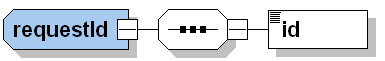
\includegraphics[width=0.45\columnwidth]{images/datatype-requestid}
		\caption{Request-ID Data Type}
		\label{fig:datatype-requestid}
	\end{figure}
	\begin{figure}[htb]
		\centering
		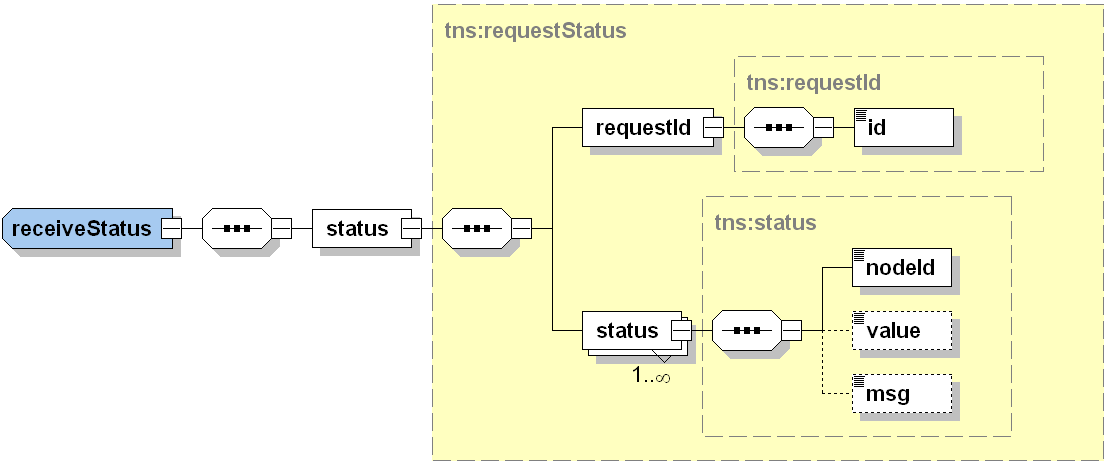
\includegraphics[width=0.9\columnwidth]{images/datatype-request-status}
		\caption{Request Status Data Type}
		\label{fig:datatype-request-status}
	\end{figure}

The status of an operation is reported to the controller via so-called status updates (of type RequestStatus) as depicted in \figref{datatype-request-status}. A status update comprises the original request identifier and a number of values for different nodes. For instance, when flashing a number of nodes at once, a status update contains full or partial information about the progress of the overall operation, i.e. information about a subset of the currently reprogrammed nodes. The controller must therefore track the progress based on potentially a number of these status updates until all nodes report completion or failure. The status update contains the node identifier, a numerical value, and a human readable message. The interpretation of the value depends on the operation and is described later for each of the operations.

%------------------------------------------------------------------------------------------------
		\subsubsection{Message Data Type}
%------------------------------------------------------------------------------------------------
The previous text-based messages are now able to convey either binary or textual data. In addition, meta data about a message (e.g., timestamp, source, type and messageLevel such as debug, error or fatal) may be present. This is shown in \figref{datatype-message}.

	\begin{figure}[htb]
		\centering
		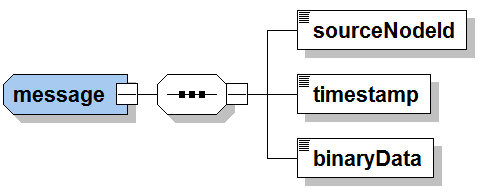
\includegraphics[width=0.95\columnwidth]{images/datatype-message}
		\caption{Message Data Type}
		\label{fig:datatype-message}
	\end{figure}

%------------------------------------------------------------------------------------------------
		\subsubsection{receiveStatus}
%------------------------------------------------------------------------------------------------

\begin{apidoc}
	{void receiveStatus(RequestStatus status[])} %Signature
	{Reports the status of an operation to the controller} % Semantics
	{
			\apiparameters{
				\apiparam{status}{The status of an operation. The content is defined by the operation that reports its status. May return an array of status indicators for a collection of previously-issued operations.}
			}
	} % Parameters
	{nothing} % Returns
	{Performance, Avoid timeouts (see above)} % Rationale for addition/changes
	{2.0} % Since
\end{apidoc}

As described above, asynchronously triggered operations send status messages about the progress or result of operations. These status messages are delivered from the Testbed Service to the controller using this operation. The operation does not return any value. The format and semantics of the values contained in the parameter "status" depend on the operation, this status messages belongs to. See the individual sections for a definition.

%------------------------------------------------------------------------------------------------
			\subsubsection{receive}
%------------------------------------------------------------------------------------------------

\begin{apidoc}
	{void receive(Message msg[])} %Signature
	{This message is invoked by the Testbed Service to convey messages from sensor nodes to the controller. The format of the parameter "msg" is described in API2.0::4.2. The operation does not return any value.
	} % Semantics
	{
			\apiparameters{
				\apiparam{msg}{The message so be received}
			}
	} % Parameters
	{nothing} % Returns
	{Changed to use the message data type, more general concept for virtual links} % Rationale for addition/changes
	{2.0
		\begin{itemize}
			\item 1.0: Initial appearance as ``deliverOutputFromSensorNode()''
			\item 2.0: Re-uses the message data type to convey messages from the Testbed Service to the Controller Service 
		\end{itemize}
	} % Since
\end{apidoc}

%------------------------------------------------------------------------------------------------
		\subsubsection{receiveNotification}
%------------------------------------------------------------------------------------------------

\begin{apidoc}
	{void receiveNotification(String notifications[])} %Signature
	{Provides a notification from the server (usually a fault or warning intended for the user)} % Semantics
	{
			\apiparameters{
				\apiparam{notifications}{An array of strings containing notifications.}
			}
	} % Parameters
	{nothing} % Returns
	{} % Rationale for addition/changes
	{2.3} % Since
\end{apidoc}

%------------------------------------------------------------------------------------------------
		\subsubsection{experimentEnded}
%------------------------------------------------------------------------------------------------

\begin{apidoc}
	{void experimentEnded()} %Signature
	{Notifies that controller that it can shut down} % Semantics
	{
	} % Parameters
	{nothing} % Returns
	{Informs controller of when it can shut down (if it wishes to) as no further communication will be made from this instance} % Rationale for addition/changes
	{2.3} % Since
\end{apidoc}